\documentclass[11pt]{article}
\usepackage[margin=1in]{geometry}
\usepackage{graphicx}
\usepackage{booktabs}
\usepackage{tabularx}
\usepackage{hyperref}

\title{ACL - Seminar 3}
\author{Ichim Ștefan}
\date{}

\begin{document}

\maketitle

Two texts from Project Gutenberg were analyzed by tokenizing them (lowercase, alphabetic characters only) and computing frequency statistics. The implementation used regular expressions (\texttt{re.findall}) for tokenization, \texttt{collections.Counter} for word frequency counting, and \texttt{matplotlib} for visualizing the frequency distributions.

\section{Hamlet}

\begin{table}[h]
\centering
\small
\begin{tabularx}{\textwidth}{|X|X|X|X|X|}
\hline
\textbf{Corpus Source} & \textbf{Tokens} & \textbf{Types} & \textbf{Top 7 Words} & \textbf{Coverage \& Hapax} \\
\hline
Hamlet by Shakespeare

\url{https://www.gutenberg.org/files/1524/1524-0.txt} & 32,789 & 4,547 & the (1112), and (986), to (735), of (680), i (635), a (561), you (559) & Top 7 coverage: 16.07\%

Words appearing once: 2632, 8.03\% of tokens, 57.88\% of types \\
\hline
\end{tabularx}
\end{table}

\begin{figure}[h]
\centering
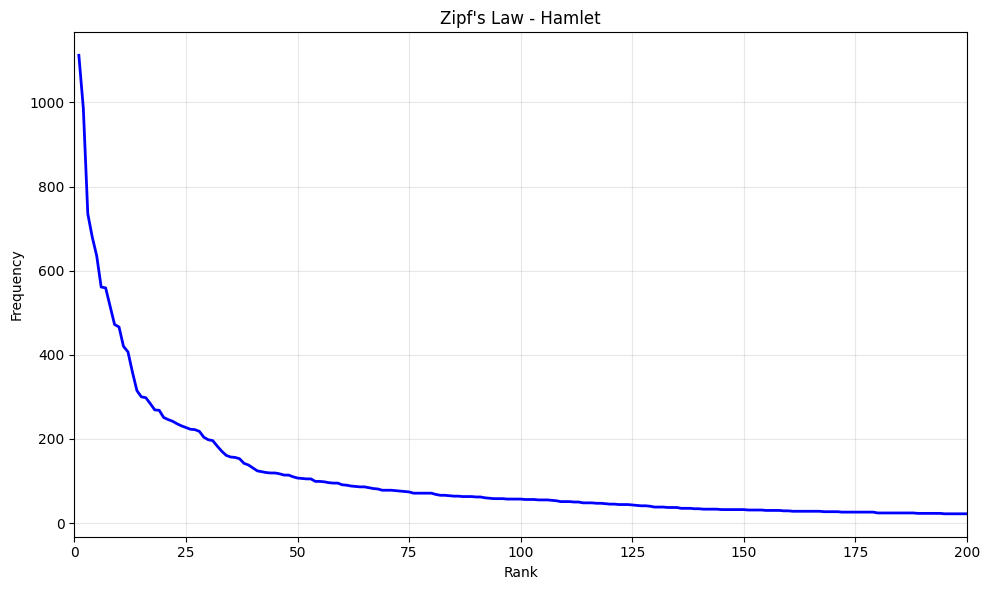
\includegraphics[width=0.65\textwidth]{zipf_hamlet.png}
\caption{Frequency distribution for Hamlet}
\end{figure}

\section{Don Quixote}

\begin{table}[h]
\centering
\small
\begin{tabularx}{\textwidth}{|X|X|X|X|X|}
\hline
\textbf{Corpus Source} & \textbf{Tokens} & \textbf{Types} & \textbf{Top 7 Words} & \textbf{Coverage \& Hapax} \\
\hline
Don Quixote by Cervantes

\url{https://www.gutenberg.org/files/996/996-0.txt} & 433,477 & 15,586 & the (22479), and (17719), to (14008), of (13493), that (7994), in (7338), a (7197) & Top 7 coverage: 20.81\%

Words appearing once: 5663, 1.31\% of tokens, 36.33\% of types \\
\hline
\end{tabularx}
\end{table}

\begin{figure}[h]
\centering
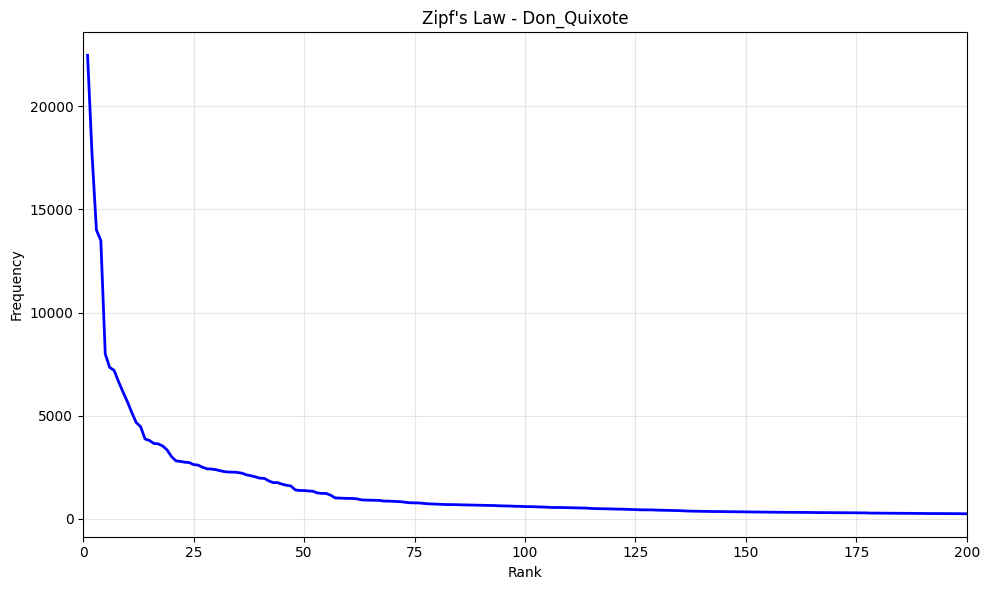
\includegraphics[width=0.65\textwidth]{zipf_don_quixote.png}
\caption{Frequency distribution for Don Quixote}
\end{figure}

\end{document}
